% Original CSC302 teaching adaptation of Heather Macbeth, The Mechanics of Proof.
% Source: https://hrmacbeth.github.io/math2001/07_Number_Theory.html
% Source snapshot: e660f42b13ddcb6d12b52ba036d6bd071a0cfb9b (Lean 4.3).
% Section 7 has unnumbered theorems; comments identify them by their names.
% Original exposition and diagrams. Lean fragments are not build-verified.
% Source correction, Section 7.3, second (integer) theorem/proof:
% prose states a^2=2b^2, while its algebra and Lean use b^2=2a^2.
% Here the statement remains a^2=2b^2, b!=0, and the swapped identity is used:
% (2*b*x+a*y)^2 = 2*(a*x+b*y)^2+(y^2-2*x^2)*(a^2-2*b^2).
% This polynomial identity was independently checked by exact symbolic expansion.
% Source correction, Section 7.3, end of natural-number prose proof:
% its final 'cannot be that a^2 != 2b^2' is replaced by the intended
% 'a^2 = 2b^2 is impossible'. The actual descent is preserved.
% CSC302 lecture slides adapted from Heather Macbeth, The Mechanics of Proof.
\documentclass[aspectratio=169,11pt]{beamer}
\usepackage[T1]{fontenc}
\usepackage{lmodern}
\usepackage{amsmath,amssymb,mathtools}
\usepackage{booktabs,array,listings,tikz}
\usetikzlibrary{arrows.meta,positioning,calc}
\definecolor{ProofNavy}{HTML}{18324F}
\definecolor{ProofTeal}{HTML}{007D82}
\definecolor{ProofPaper}{HTML}{F3F6F8}
\usetheme{default}
\setbeamercolor{normal text}{fg=ProofNavy,bg=white}
\setbeamercolor{structure}{fg=ProofTeal}
\setbeamercolor{frametitle}{fg=ProofNavy}
\setbeamercolor{block title}{fg=white,bg=ProofNavy}
\setbeamercolor{block body}{fg=ProofNavy,bg=ProofPaper}
\setbeamercolor{block title example}{fg=white,bg=ProofTeal}
\setbeamercolor{block body example}{fg=ProofNavy,bg=ProofPaper}
\setbeamerfont{frametitle}{size=\Large,series=\bfseries}
\setbeamertemplate{navigation symbols}{}
\setbeamertemplate{itemize item}{\small\textbullet}
\setbeamertemplate{footline}{%
  \leavevmode\hbox{%
  \begin{beamercolorbox}[wd=.86\paperwidth,ht=2.8ex,dp=1.2ex,leftskip=1.6em]{author in head/foot}%
    \scriptsize CSC302\quad\textbar\quad\insertshorttitle
  \end{beamercolorbox}%
  \begin{beamercolorbox}[wd=.14\paperwidth,ht=2.8ex,dp=1.2ex,rightskip=1.6em plus1fil]{date in head/foot}%
    \scriptsize\insertframenumber/\inserttotalframenumber
  \end{beamercolorbox}}}
\setbeamersize{text margin left=8mm,text margin right=8mm}
\lstdefinelanguage{Lean}{%
  morekeywords={example,theorem,lemma,def,by,calc,have,exact,apply,intro,intros,constructor,rcases,rfl,rw,ring,numbers,linarith,nlinarith,rel,extra,addarith,obtain,left,right,use,choose,dsimp,change,ext,fun,show,from,at,with,induction,case,decide,contradiction,push_neg,by_cases,by_contra,assumption,existsi,simp,simpa},
  sensitive=true,morecomment=[l]{--},morestring=[b]"}
\lstset{language=Lean,basicstyle=\ttfamily\small,keywordstyle=\color{ProofTeal}\bfseries,
  commentstyle=\color{gray},stringstyle=\color{ProofNavy},showstringspaces=false,
  columns=fullflexible,keepspaces=true,breaklines=true,frame=single,
  rulecolor=\color{ProofTeal!30},backgroundcolor=\color{ProofPaper},
  aboveskip=0.5em,belowskip=0.4em}
\newcommand{\N}{\mathbb{N}}
\newcommand{\Z}{\mathbb{Z}}
\newcommand{\Q}{\mathbb{Q}}
\newcommand{\R}{\mathbb{R}}
\newcommand{\coursechapter}[2]{%
  \title[Chapter #1: #2]{Chapter #1\\#2}%
  \subtitle{The Mechanics of Proof \textbar{} CSC302 lecture notes}%
  \author{Based on Heather Macbeth's textbook}%
  \date{}%
}
\newcommand{\sourcecredit}[1]{\par\vfill{\tiny Source: Heather Macbeth, \emph{The Mechanics of Proof}, #1.}}
\newcommand{\bookurl}{\url{https://hrmacbeth.github.io/math2001/}}
\hypersetup{colorlinks=true,urlcolor=ProofTeal,linkcolor=ProofNavy}

\coursechapter{7}{Number theory}
\begin{document}
\begin{frame}\titlepage\end{frame}

\begin{frame}{What you should be able to do}
\begin{itemize}
\item Explain why a prime divisor of $N!+1$ must exceed $N$.
\item Use a B\'ezout identity to justify cancellation in divisibility.
\item Derive Euclid's lemma from the defining property of a prime.
\item Identify the decreasing positive integer in an infinite-descent proof.
\item Connect an integer equation to irrationality.
\end{itemize}
\begin{block}{Capstone perspective}
The new results combine familiar tools: witnesses, case splits, induction, gcd, and contradiction. Each proof also needs a specific mathematical construction.
\end{block}
\sourcecredit{Chapter 7, Sections 7.1--7.3}
\end{frame}

% Chapter 7 introduction; prerequisites from 4.1.8, 6.2.5, 6.4.2, 6.7.6.
\begin{frame}{A map of the ingredients}
\begin{center}
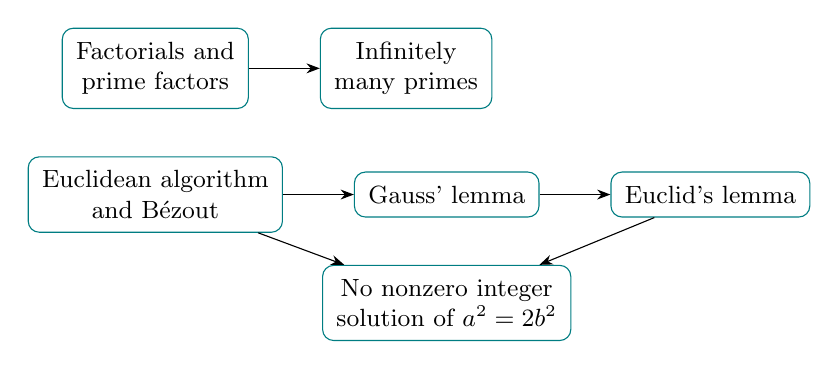
\begin{tikzpicture}[>=Stealth,node distance=6mm and 9mm,
 every node/.style={draw=ProofTeal,rounded corners,align=center,font=\small,inner sep=5pt}]
\node (fac) {Factorials and\\prime factors};
\node[right=of fac] (inf) {Infinitely\\many primes};
\node[below=of fac] (bez) {Euclidean algorithm\\and B\'ezout};
\node[right=of bez] (gauss) {Gauss' lemma};
\node[right=of gauss] (euclid) {Euclid's lemma};
\node[below=of gauss] (sqrt) {No nonzero integer\\solution of $a^2=2b^2$};
\draw[->] (fac)--(inf);
\draw[->] (bez)--(gauss);
\draw[->] (gauss)--(euclid);
\draw[->] (euclid)--(sqrt);
\draw[->] (bez)--(sqrt);
\end{tikzpicture}
\end{center}
For the descent proof, the needed parity fact can also be obtained directly from Chapter 6.
\sourcecredit{Chapter 7; prerequisites in Sections 6.2, 6.4, and 6.7}
\end{frame}

\section{7.1 Infinitely many primes}
% Section 7.1, unnumbered theorem. The strengthened p>N conclusion is in its proof.
\begin{frame}{7.1: What does it mean to have infinitely many primes?}
\begin{block}{Prime}
A natural number $p$ is prime if $p\ge2$ and each natural divisor of $p$ is either $1$ or $p$.
\end{block}
We will prove the concrete statement
\[
\forall N\in\N,\quad\exists p\in\N,\quad p>N\text{ and }p\text{ is prime}.
\]
Why is that enough? Any finite list of natural numbers has an upper bound $N$. The theorem supplies a prime outside that list.
\medskip
The construction will produce a \emph{prime factor} of a new number, rather than require that the new number itself be prime.
\sourcecredit{Section 7.1, theorem on infinitely many primes; definition from 4.1.8}
\end{frame}

% Section 7.1, factorial construction; references 6.2.5 and 6.4.2.
\begin{frame}{Build a number with a prime factor}
Fix an arbitrary $N\in\N$ and put $M=N!$.
\begin{enumerate}
\item $M\ge1$, so $M+1\ge2$.
\item Every natural number at least $2$ has a prime factor. Choose a prime $p$ with $p\mid M+1$.
\item Write $M+1=pk$ with $k\in\N$.
\item Since $M+1>0$, $k\ne0$. Write $k=\ell+1$ with $\ell\in\N$.
\end{enumerate}
We now know
\[
p\ge2,\qquad M+1=p(\ell+1).
\]
The next step will prove that $p$ cannot also divide $M$.
\sourcecredit{Section 7.1; uses factorial positivity and the prime-factor theorem}
\end{frame}

% Section 7.1, consecutive-multiples argument, keeping the source's Nat route.
\begin{frame}{The new prime factor is larger than the bound}
From $M+1=p(\ell+1)=p\ell+p$ and $p\ge2$, we get
\[
p\ell<M<p(\ell+1).
\]
Thus $M$ lies strictly between consecutive multiples of $p$, so $p\nmid M$.
\begin{enumerate}
\item Suppose $p\le N$.
\item Since $1\le p\le N$, the factorial-divisibility theorem gives $p\mid N!=M$.
\item This contradicts $p\nmid M$.
\end{enumerate}
Therefore $p>N$. Since $N$ was arbitrary, there are infinitely many primes.
\sourcecredit{Section 7.1; uses Examples 4.5.8 and 6.2.5}
\end{frame}

% Original concrete illustrations of Section 7.1; arithmetic independently checked.
\begin{frame}{The construction can start with a composite number}
\begin{center}
\begin{tabular}{ccll}
\toprule
$N$ & $N!+1$ & Prime factor $p$ & Comparison\\\midrule
$4$ & $25=5^2$ & $5$ & $5>4$\\[2mm]
$5$ & $121=11^2$ & $11$ & $11>5$\\[2mm]
$6$ & $721=7\cdot103$ & $7$ & $7>6$\\\bottomrule
\end{tabular}
\end{center}
\begin{block}{What the theorem needs}
The integer $N!+1$ only needs to be at least $2$ so that it has a prime divisor. Every such prime divisor exceeds $N$.
\end{block}
The proof gives a new prime beyond a chosen bound; it does not claim that factorial-plus-one is always prime.
\sourcecredit{Section 7.1; original numerical illustrations}
\end{frame}

% Section 7.1 classroom extensions: boundary N=0 and finite-product Euclid proof.
\begin{frame}{7.1 Practice: explain the construction's logic}
\begin{enumerate}
\item Run the proof for $N=0$. What are $N!+1$ and its prime factor?
\item Suppose $p_1,\ldots,p_r$ is a nonempty finite list containing every prime. Set
\[
K=p_1p_2\cdots p_r+1.
\]
Explain why a prime divisor of $K$ cannot belong to the list.
\end{enumerate}
You may use: if an integer divides two integers, it divides their difference.
\sourcecredit{Section 7.1; classroom extensions of its construction}
\end{frame}

\begin{frame}{7.1 Solution ideas}
\begin{enumerate}
\item $0!=1$, so $0!+1=2$. The prime $2$ is larger than $0$; no special exception is needed.
\item $K\ge2$, so choose a prime $q\mid K$. If $q=p_i$ for some listed prime, then $q$ divides $p_1\cdots p_r$ as well. Hence
\[
q\mid\bigl(K-p_1\cdots p_r\bigr)=1,
\]
which is impossible for $q\ge2$.
\end{enumerate}
The factorial version excludes every prime up to $N$; the product version excludes every prime in the given list.
\sourcecredit{Section 7.1; solutions to the preceding extensions}
\end{frame}

\section{7.2 Gauss' and Euclid's lemmas}
% Section 7.2, Gauss' lemma, over integers with no unnecessary sign restriction.
\begin{frame}{7.2: When may a factor be cancelled in divisibility?}
\begin{block}{Gauss' lemma}
Let $a,b,d\in\Z$. If
\[
d\mid ab\qquad\text{and}\qquad\gcd(a,d)=1,
\]
then $d\mid b$.
\end{block}
The condition $\gcd(a,d)=1$ says that $a$ and $d$ are coprime.
\begin{block}{Why the hypothesis matters}
$6\mid2\cdot3$, but $6\nmid3$. Here $\gcd(2,6)=2$, so the coprimality assumption fails.
\end{block}
B\'ezout's identity will express $1$ as a combination of $a$ and $d$.
\sourcecredit{Section 7.2, Gauss' lemma; counterexample is an extension}
\end{frame}

% Section 7.2, Gauss proof. Coefficients and witness kept explicit.
\begin{frame}{Gauss' lemma: construct the divisibility witness}
Choose $x,y\in\Z$ with $xa+yd=1$, using B\'ezout and $\gcd(a,d)=1$.
Choose $z\in\Z$ with $ab=dz$, using $d\mid ab$.
Then
\[
\begin{aligned}
b&=b(xa+yd)\\
 &=x(ab)+byd\\
 &=x(dz)+byd\\
 &=d(xz+by).
\end{aligned}
\]
Thus $xz+by\in\Z$ witnesses $d\mid b$.
\begin{block}{Lean connection}
\texttt{obtain} extracts the B\'ezout coefficients and divisibility witness; \texttt{use} supplies the new witness; \texttt{rw} and \texttt{ring} verify the calculation.
\end{block}
\sourcecredit{Section 7.2, proof of Gauss' lemma}
\end{frame}

% Original worked instance of Gauss' lemma; 3*12-35=1 verified.
\begin{frame}{A concrete cancellation problem}
Let $n\in\Z$ and suppose $35\mid12n$. Prove $35\mid n$.
\begin{enumerate}
\item The identity $3\cdot12-35=1$ supplies the needed coprimality information.
\item Write $12n=35k$ with $k\in\Z$.
\item Multiply the identity by $n$:
\[
\begin{aligned}
n&=3(12n)-35n\\
 &=3(35k)-35n\\
 &=35(3k-n).
\end{aligned}
\]
\end{enumerate}
The proof not only shows divisibility; it gives a quotient $3k-n$.
\sourcecredit{Section 7.2, Gauss' lemma; original worked instance}
\end{frame}

% Section 7.2, Euclid's lemma and gcd-case proof.
\begin{frame}{Euclid's lemma: primes divide one factor}
\begin{block}{Theorem}
For $a,b,p\in\N$, if $p$ is prime and $p\mid ab$, then $p\mid a$ or $p\mid b$.
\end{block}
Put $d=\gcd(a,p)$. We know $d\mid a$ and $d\mid p$.
Since $p$ is prime, $d=1$ or $d=p$.
\begin{center}
\begin{tabular}{ll}
\toprule
Case & Conclusion\\\midrule
$d=1$ & Gauss' lemma applied to $p\mid ab$ gives $p\mid b$.\\[2mm]
$d=p$ & Since $d\mid a$, we have $p\mid a$.\\\bottomrule
\end{tabular}
\end{center}
Primality reduces the gcd to exactly the two cases needed by the proof.
\sourcecredit{Section 7.2, Euclid's lemma}
\end{frame}

% Section 7.2, power corollary. Preserve k>=1.
\begin{frame}{A prime divisor of a power divides the base}
Let $a,p,k\in\N$, with $p$ prime and $k\ge1$. Then
\[
p\mid a^k\quad\Longrightarrow\quad p\mid a.
\]
Prove this by induction on $k$, starting at $1$.
\begin{itemize}
\item \textbf{Base:} $a^1=a$.
\item \textbf{Step:} if $p\mid a^{t+1}=a\cdot a^t$, Euclid's lemma gives $p\mid a$ or $p\mid a^t$. The first case finishes; the second uses the inductive hypothesis.
\end{itemize}
\begin{block}{A consequence we will use}
If $a^2$ is even, then $a$ is even: apply the result with the prime $p=2$ and $k=2$.
\end{block}
\sourcecredit{Section 7.2, power corollary}
\end{frame}

% Section 7.2, paragraph preceding Lean Euclid proof (casts, lift, norm_cast).
\begin{frame}{Lean keeps the integer and natural-number statements separate}
The textbook defines its gcd on $\Z$, while its prime predicate is on $\N$.
\begin{enumerate}
\item Cast $a$ and $p$ to integers to apply gcd and Gauss' lemmas.
\item Use $\gcd(a,p)\ge0$ to represent that integer gcd by a natural number $d$.
\item Transfer the divisibility facts to $\N$, where the prime definition applies.
\end{enumerate}
\begin{center}
\begin{tabular}{ll}
\toprule
Textbook notation/tactic & Purpose\\\midrule
\texttt{(a : Int)} & View a natural number as an integer.\\
\texttt{lift} & Replace a nonnegative integer by a natural number.\\
\texttt{norm\_cast} & Transport compatible statements across casts.\\\bottomrule
\end{tabular}
\end{center}
The mathematical case split remains $d=1$ or $d=p$.
\sourcecredit{Section 7.2, Lean discussion following Euclid's lemma}
\end{frame}

% Original classroom applications of Gauss/Euclid/power corollary.
\begin{frame}{7.2 Practice: choose the correct divisibility tool}
\begin{enumerate}
\item Let $n\in\Z$ and $9\mid4n$. Use $7\cdot4-3\cdot9=1$ to produce a witness for $9\mid n$.
\item Let $u,v\in\N$. If $7\mid u^2v$ and $7\nmid u$, prove $7\mid v$.
\item Find a composite $d$ and natural $a,b$ such that $d\mid ab$, but $d\nmid a$ and $d\nmid b$.
\end{enumerate}
Name every primality or coprimality hypothesis used in your proof.
\sourcecredit{Section 7.2; original classroom exercises}
\end{frame}

\begin{frame}{7.2 Solution ideas}
\begin{enumerate}
\item Write $4n=9k$. Then
\[
n=7(4n)-27n=9(7k-3n).
\]
So $7k-3n$ is a witness.
\item Euclid's lemma gives $7\mid u^2$ or $7\mid v$. The first case implies $7\mid u$ by the power corollary, contradicting the hypothesis. Hence $7\mid v$.
\item Take $d=6$, $a=2$, and $b=3$. This shows why Euclid's lemma requires a prime divisor.
\end{enumerate}
\sourcecredit{Section 7.2; solutions to the preceding exercises}
\end{frame}

\section{7.3 The square root of two}
% Section 7.3, first theorem, natural-number strong-induction proof.
\begin{frame}{7.3: The arithmetic statement behind irrationality}
\begin{block}{Theorem}
There are no $a,b\in\N$ with $b\ne0$ such that $a^2=2b^2$.
\end{block}
The assumption $b\ne0$ is essential: $(a,b)=(0,0)$ satisfies the equation.
\medskip
We will prove by strong induction on $b$ the property
\[
P(b):\quad\forall a\in\N,\quad b\ne0\Rightarrow a^2\ne2b^2.
\]
\begin{block}{Why quantify over all numerators?}
The next solution will have a different numerator. The induction hypothesis must cover every $a$ at each smaller denominator.
\end{block}
\sourcecredit{Section 7.3, natural-number theorem and descent proof}
\end{frame}

% Section 7.3, descent construction. Even-square lemma supplied by 7.2.
\begin{frame}{From one hypothetical solution, build a smaller one}
Suppose $a,b\in\N$, $b\ne0$, and $a^2=2b^2$.
\begin{enumerate}
\item $2\mid a^2$, so $2\mid a$. Write $a=2k$ for some $k\in\N$.
\item Substitute and cancel the nonzero factor $2$:
\[
2b^2=a^2=(2k)^2=4k^2
\quad\Longrightarrow\quad b^2=2k^2.
\]
\item Thus $(b,k)$ satisfies the same form of equation as $(a,b)$.
\end{enumerate}
\begin{block}{The remaining obligations}
To use the induction hypothesis, we must prove $k\ne0$ and $k<b$. A new solution alone does not yet give a contradiction.
\end{block}
\sourcecredit{Section 7.3, natural-number descent; parity fact also follows from 7.2}
\end{frame}

% Section 7.3, irrat_aux_wf and the termination argument.
\begin{frame}{Check the denominator really decreases}
We have $b\ne0$ and $b^2=2k^2$.
\begin{enumerate}
\item If $k=0$, then $b^2=0$, hence $b=0$, a contradiction. Thus $k>0$.
\item Since $k^2>0$,
\[
k^2<2k^2=b^2.
\]
Because $k,b\ge0$, this implies $k<b$.
\item The strong-induction hypothesis at denominator $k$, with numerator $b$, says $b^2\ne2k^2$.
\end{enumerate}
This contradicts the new equation. Therefore the assumed original solution cannot exist.
\sourcecredit{Section 7.3, well-foundedness lemma and natural-number proof}
\end{frame}

% Section 7.3, irrat_aux and termination_by; local proof fragment is an adaptation.
\begin{frame}[fragile]{The precise role of the induction hypothesis}
At denominator $b$, the hypothesis covers \emph{all} pairs $(r,s)$ with $s<b$:
\[
\forall r,s\in\N,\quad s<b\Rightarrow s\ne0\Rightarrow r^2\ne2s^2.
\]
Once the preceding slides supply $k<b$, $k\ne0$, and $b^2=2k^2$:
\begin{lstlisting}
-- Local demonstration fragment in the induction step:
-- IH covers every numerator r at every denominator s < b.
-- hkb : k < b; hk : Not (k = 0)
-- hnew : b ^ 2 = 2 * k ^ 2
have forbidden := IH b k hkb hk
exact forbidden hnew
\end{lstlisting}
The textbook expresses this as a recursive theorem call, with termination measured by the second argument.
\sourcecredit{Section 7.3, theorem irrat\_aux and its termination explanation}
\end{frame}

% Section 7.3, second theorem. Corrected orientation documented at file header.
\begin{frame}{A second proof: use gcd and B\'ezout}
Now let $a,b\in\Z$ with $b\ne0$, and suppose $a^2=2b^2$.
Put $d=\gcd(a,b)$.
\begin{enumerate}
\item Since $d\mid a$ and $d\mid b$, choose $k,\ell\in\Z$ with
\[
a=dk,\qquad b=d\ell.
\]
\item B\'ezout gives $x,y\in\Z$ with $ax+by=d$.
\item $d\ne0$: otherwise $b=d\ell=0$, a contradiction.
\end{enumerate}
We will construct an integer $z$ with $z^2=2$, which is impossible.
\sourcecredit{Section 7.3, integer theorem and B\'ezout proof; notation normalized}
\end{frame}

% Section 7.3, Brahmagupta identity step; exact polynomial expansion checked.
\begin{frame}{The key identity creates an integer square root of 2}
Set $z=2\ell x+ky\in\Z$. Then
\[
\begin{aligned}
d^2z^2
  &=(2bx+ay)^2\\
  &=2(ax+by)^2+(y^2-2x^2)(a^2-2b^2)\\
  &=2d^2+(y^2-2x^2)\cdot0\\
  &=2d^2.
\end{aligned}
\]
The middle equality is a polynomial identity, verified by expansion.
Since $d\ne0$, cancellation of $d^2$ gives $z^2=2$.
\begin{block}{Where each input was used}
$a=dk$, $b=d\ell$: first line.\quad $ax+by=d$: third line.\quad
$a^2=2b^2$: third line.\quad $d\ne0$: cancellation.
\end{block}
\sourcecredit{Section 7.3, integer proof using Brahmagupta's identity}
\end{frame}

% Section 7.3 cites Example 2.3.5 (no integer square is two).
\begin{frame}{Why the integer square equation is impossible}
If $z\in\Z$, then $|z|$ is a nonnegative integer. Exactly one of the following ranges applies:
\begin{center}
\begin{tabular}{ll}
\toprule
Range & Bound on $z^2$\\\midrule
$|z|\le1$ & $z^2=|z|^2\le1<2$\\[2mm]
$|z|\ge2$ & $z^2=|z|^2\ge4>2$\\\bottomrule
\end{tabular}
\end{center}
Thus $z^2\ne2$ for every integer $z$, contradicting the constructed $z$.
\begin{block}{Conclusion of the second proof}
There are no integers $a,b$ with $b\ne0$ and $a^2=2b^2$.
\end{block}
\sourcecredit{Section 7.3, completion of the integer proof; prerequisite Example 2.3.5}
\end{frame}

% Explicit extension: the source defers the formal definition of rationals.
\begin{frame}{Extension: translating the equation into irrationality}
A real number is \emph{rational} when it can be written $a/b$ with $a,b\in\Z$ and $b\ne0$. A real number that is not rational is \emph{irrational}.
\medskip
Suppose a rational $q=a/b$ satisfied $q^2=2$. Multiplication by $b^2$ would give
\[
a^2=2b^2,
\]
contradicting the integer theorem.
\begin{block}{Consequence}
Every real solution of $q^2=2$ is irrational. In particular, the positive solution $\sqrt2$ is irrational.
\end{block}
No assumption that $a/b$ is in lowest terms is needed by these proofs.
\sourcecredit{Section 7.3, arithmetic theorem; rational-number interpretation added for CSC302}
\end{frame}

% Original classroom applications of the two source proofs.
\begin{frame}{7.3 Practice: audit a descent argument}
\begin{enumerate}
\item In the natural-number proof, explain why the induction hypothesis must allow a numerator different from the original $a$.
\item A proposed proof produces another solution $(a',b')$ but only shows $b'\le b$. Explain why this does not finish a descent argument.
\item Adapt the descent proof to show that no natural $a,b$ with $b\ne0$ satisfy $a^2=3b^2$. You may use Euclid's lemma for the prime $3$.
\end{enumerate}
For item 3, list the new pair and prove both required inequalities about its denominator.
\sourcecredit{Section 7.3; original proof-audit and generalization exercises}
\end{frame}

\begin{frame}{7.3 Solution ideas}
\begin{enumerate}
\item The new pair is $(b,k)$, so the numerator changes from $a$ to $b$. The induction property is quantified over every numerator.
\item A process may repeat the same denominator forever. Strong induction requires a \emph{strictly} smaller nonnegative integer.
\item From $3\mid a^2$, obtain $a=3k$. Then
\[
a^2=3b^2\Rightarrow9k^2=3b^2\Rightarrow b^2=3k^2.
\]
Here $k\ne0$ because $b\ne0$, and $k^2<3k^2=b^2$ gives $k<b$. The pair $(b,k)$ contradicts the induction hypothesis at $k$.
\end{enumerate}
\sourcecredit{Section 7.3; solutions to the preceding exercises}
\end{frame}

\begin{frame}{Review: the construction and the reason it works}
\begin{center}
\begin{tabular}{p{.25\textwidth}p{.31\textwidth}p{.32\textwidth}}
\toprule
Result & Construction & Decisive fact\\\midrule
Infinitely many primes & Prime divisor of $N!+1$ & It cannot divide $N!$.\\[2mm]
Gauss' lemma & Multiply a B\'ezout identity by $b$ & An explicit multiple of $d$ results.\\[2mm]
Euclid's lemma & Examine $\gcd(a,p)$ & A prime has only two natural divisors.\\[2mm]
No $a^2=2b^2$, $b\ne0$ & Smaller solution, or an integer square root of $2$ & Strict descent, or the gap between $1$ and $4$.\\\bottomrule
\end{tabular}
\end{center}
In every proof, identify the witness, preserve its domain, and check the assumption that permits cancellation or induction.
\sourcecredit{Chapter 7, Sections 7.1--7.3}
\end{frame}

\begin{frame}{Sources and further work}
Heather Macbeth, \emph{The Mechanics of Proof}, Chapter 7.
\begin{itemize}
\item 7.1: factorial construction for infinitely many primes.
\item 7.2: Gauss' lemma, Euclid's lemma, and the power corollary.
\item 7.3: the natural-number descent and integer B\'ezout proofs.
\end{itemize}
\medskip
\href{https://hrmacbeth.github.io/math2001/07_Number_Theory.html}{Read Chapter 7 and compare the mathematical and Lean proofs.}
\medskip

The prose, diagrams, and classroom exercises in this deck are original adaptations. The rational-number interpretation is an explicit extension. Lean fragments use the textbook's educational environment.
\end{frame}
\end{document}
